\chapter{Results and Interpretations}

\section{Observation vs Predicted}
This is where I'll put the tables for the observed and predicted number of events in each search region bin.

\section{Simplified models}
The interpretation of these results uses the T5gg and T6gg simplified models.  The T5gg simplified model gluino ($\tilde{g}$) pair production while the T6gg model assumes squark ($\tilde{q}$) pair production. The lightest supersymmetric particle (LSP) in both models is the gravitino $\tilde{G}$ and the next-to-lightest supersymmetric particle is the neutralino $\tilde{\chi}^{0}_{1}$.  Figure \ref{fig:susysignals} shows examples of decay chains for both models.  

Monte Carlo scans were used to evaluate the expected signal distributions for these models.  The scan for the T5gg model was produced in bins of gluino and neutralino masses while the T6gg scan was binned in squark and neutralino masses.  $\verb|MadGraph5_aMC@NLO|$ was used for event generation\cite{Alwall:2014hca} while $\verb|PYTHIA 8|$ was used for simulating parton showering, hadronization, and multi-parton interactions\cite{Sjostrand:2007gs}.  The detector response was simulated with CMS fast simulation\cite{Abdullin:2011zz}.  Production cross sections were calculated next-to-leading order (NLO) plus next-to-logarithmic (NLL) accuracy \cite{Borschensky:2014cia}.  For calculations of gluino cross sections the squark was taken to be heavy and decoupled and vice versa for squark cross section calculations.  The cross sections for gluino and squark pair production are shown in Figures \ref{fig:gluinoxsec} and \ref{fig:squarkxsec} respectively.

\begin{figure}[h]
	\centering
	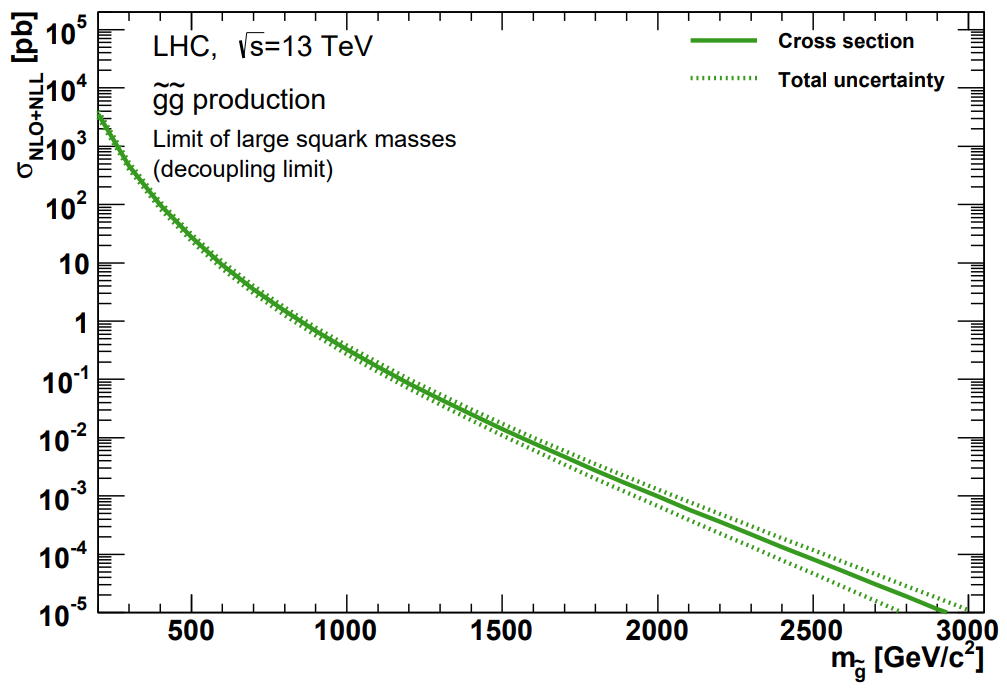
\includegraphics[width=0.9\linewidth]{Figures/gluinoxsec}
	\caption[Theoretical cross section gluino pair production as a function of gluino mass]{The NLO+NLL cross section for gluino pair production as a function of gluino mass.}
	\label{fig:gluinoxsec}
\end{figure}

\begin{figure}[h]
	\centering
	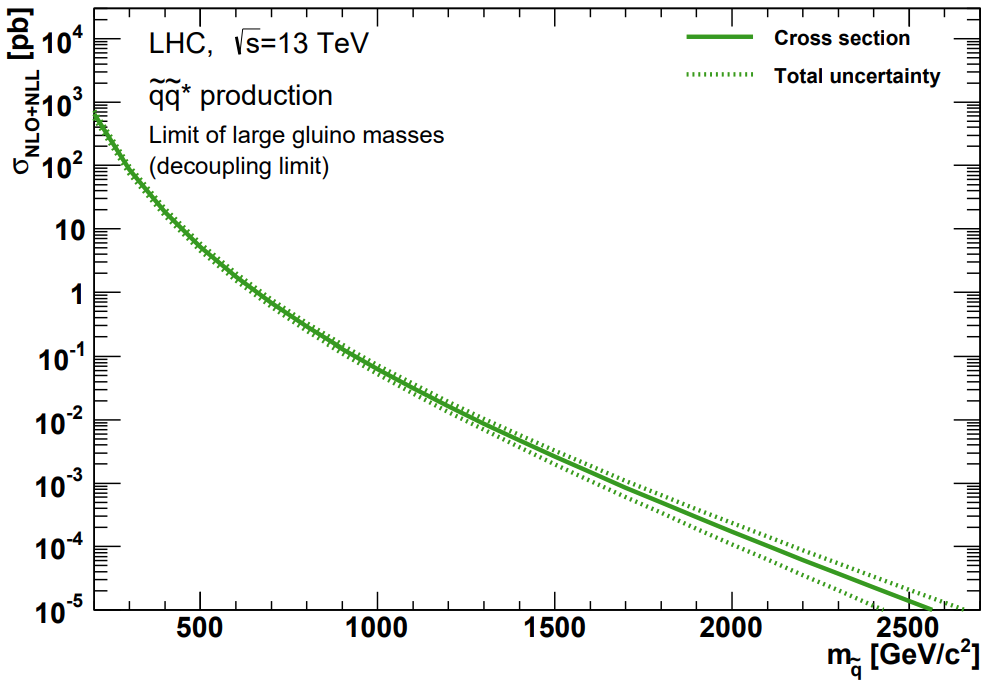
\includegraphics[width=0.9\linewidth]{Figures/squarkxsec}
	\caption[Theoretical cross section for squark pair production as a function of squark mass]{The NLO+NLL cross section for squark pair production as a function of squark mass.}
	\label{fig:squarkxsec}
\end{figure}



\section{Statistical analysis}
Upper limits for the production cross section of each signal model are evaluated using the modified frequentist method, CL$_s$, with a profile likelihood test statistic.  The uncertainties that affect the predicted signal and background yields, $s$ and $b$ respectively, are incorporated by introducing nuisance parameters $\theta$.  We can then express the signal and background expectations as functions of the nuisance parameters.  The probability $P$ for a given search region to contain $n$ observed events when expecting to observe $b$ background events and $s$ signal events can be expressed with signal strength modifier $\mu$ and the set of nuisance parameters $\theta$ as a Poisson distribution as shown in Equation \ref{eqn:Poisson}.  
\begin{equation}
	P(n|\mu , \theta) = \frac{(\mu s(\theta)+b(\theta))^{n}}{n!}e^{-(\mu s(\theta) + b(\theta))}
	\label{eqn:Poisson}
\end{equation}
The probability distribution $p_i(\theta)$ for each nuisance parameter $\theta_i$ depends on the uncertainty that it represents.  For statistical uncertainties the probability distribution is modeled with a gamma density distribution, while systematic uncertainties are modeled using a log-normal density distribution.

Combining all of the search regions we can make a likelihood function $\mathcal{L}$, which is the probability to have signal strength $\mu$ and the set of nuisance parameters $\theta$ given $n_i$ events are observed observed in search region $i$.
\begin{equation}
	\mathcal{L}(n|\mu,\theta) = \prod_{i}P(n_i|\mu, \theta)\prod_{j}p_j(\theta)
\end{equation} 
We then get the best fit values for $\mu$ and $\theta$, which will be represented by $\hat{\mu}$ and $\hat{\theta}$, by maximizing $\mathcal{L}$.  The test statistic $t_\mu$ is then used to quantify the compatibility of a given value of signal strength $\mu$ with the observed data.  That test statistic is defined as
\begin{equation}
	t_\mu = -2\ln \frac{\mathcal{L}(n|\mu, \tilde{\theta})}{\mathcal{L}(n|\hat{\mu}, \hat{\theta})} = -2\ln \frac{\mathcal{L}_\mu}{\mathcal{L}_{max}}
\end{equation}
where $\tilde{\theta}$ is the nuisance parameter set with values that maximize $\mathcal{L}$ for a given value of $\mu$.  The ratio inside the natural log is essentially the maximum likelihood with fixed $\mu$ divided by the maximum likelihood.  The best fit values for these nuisance parameters $\hat{\theta}_\mu$ are then used to generate toy MC pseudo-data in order to construct probability distributions for the background-only case, where we set $\mu=0$, and the signal+background case.  This gives the p-values for each hypothesis in terms of the a comparison between the value of test statistic resulting from the MC generated pseudo-data ($t_\mu$) and the one resulting from observed data ($t_\mu^{obs}$) as follows:
\begin{eqnarray}
	p_\mu = P(t_\mu \geq t_\mu^{obs}|signal + background) \\
	1-p_0 = P(t_0 \geq t_0^{obs}|background-only)
\end{eqnarray} 
Using the CL$_s$ method, as described in \cite{Junk:1999kv} and \cite{Read:2002hq}, we have the Confidence Level 
\begin{equation}
	CL_s(\mu) = \frac{p_\mu}{1-p_0}.
\end{equation}

By adjusting $\mu$ until $CL_s = 0.05$ we get an upper limit on the signal strength $\mu^{95\%CL}$ for a particular model with a 95\% Confidence Level.  We would then say that any model for which $CL_s \leq 0.05$ is excluded.  The cross section upper limit for model would then be the product of $\mu^{95\%CL}$ and the expected cross section of that model.  This process yields the observed cross section upper limit as it uses real observed data being plugged into the test statistic $t_\mu$.  If instead we use background prediction we would get the expected cross section upper limits.  Essentially, the expected upper limit is what we expect the find if there is no signal present, i.e. the background-only hypothesis is true.

\section{Limits for T5gg and T6gg}
The upper limits placed on production cross sections and the exclusion contours are shown in Figures \ref{fig:t5wgjul20xsec} and \ref{fig:t6wgjul20xsec} for the T5gg and T6gg simplified models respectively.  The signal models in which the 95\% CL upper limit on production cross section is less than the theoretical cross section are considered to be excluded.  These excluded signal models are to the left of the exclusion contour.  As discussed in the previous section, the expected limit exclusion contour tells us what the region of phase space we can expect to exclude if there is no signal present and everything we observe is processed consistent with the Standard Model.  The observed limit exclusion contour tells us what region of phase space is excluded given the data that we observed.
\begin{figure}[h]
	\centering
	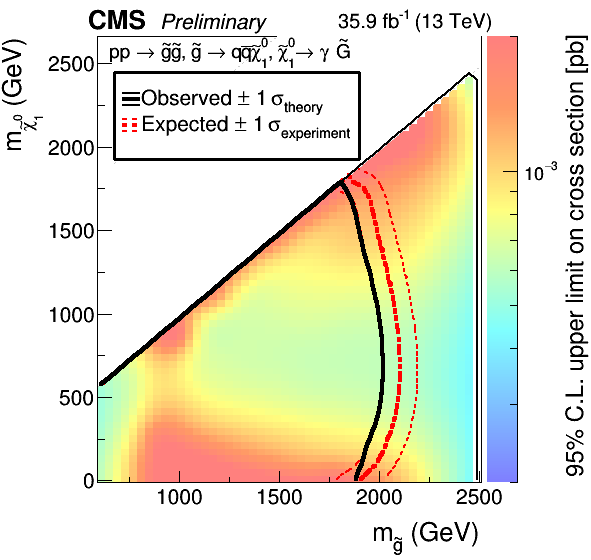
\includegraphics[width=0.9\linewidth]{Figures/T5limit_sept30}
	\caption[Cross section limits for T5gg simplified model.]{Cross section limits for T5gg simplified model.  The expected limit (black) is set by assuming that the observed data is consistent with the background-only model.  Observed data in from the signal regions is not used in the calculation of the expected limit.  The observed limit (red) is set using observed data from the signal regions.}
	\label{fig:t5wgjul20xsec}
\end{figure}
\begin{figure}[h]
	\centering
	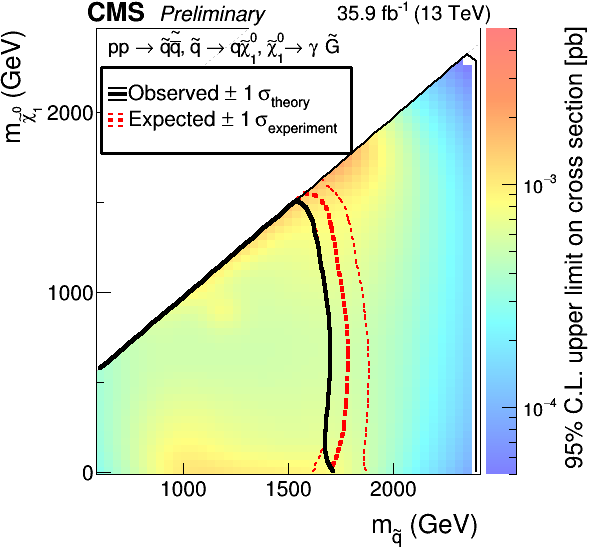
\includegraphics[width=0.9\linewidth]{Figures/T6limit_sept30}
	\caption[Cross section upper limits for T6gg simplified model.]{Cross section upper limits for T6gg simplified model.The expected limit (black) is set by assuming that the observed data is consistent with the background-only model.  Observed data in from the signal regions is not used in the calculation of the expected limit.  The observed limit (red) is set using observed data from the signal regions.}
	\label{fig:t6wgjul20xsec}
\end{figure}




